\section{数据集与评价}
\begin{frame}[allowframebreaks]
    \frametitle{\textsc{目录}} \vspace{-0.3cm}
    \begin{spacing}{0.0}
        \tableofcontents[currentsection,hideallsubsections]
    \end{spacing}   % 若不想要目录, 注释掉该句
\end{frame}

\begin{frame}
    \noindent\large\textbf{目标检测公共数据集}\\
    \vspace{1em}

    Pascal VOC,ILSVRC,MS-COCO,和Open Images 数据集是目标检测使用最多的四大公共数据集
    \vspace{2em}
    \begin{tabular}{rl}
        \small{PASCAL VOC}:  & \small{http://host.robots.ox.ac.uk/pascal/VOC/}                  \\
        \small{ILSVRC}:      & \small{https://www.image-net.org/challenges/LSVRC/}              \\
        \small{MS-COCO}:     & \small{https://cocodataset.org/\#home}                           \\
        \small{Open Images}: & \small{https://storage.googleapis.com/openimages/web/index.html} \\
    \end{tabular}
    \vspace{2em}
    本课程使用COCO-2017数据集作为示例.
\end{frame}

\begin{frame}
    \noindent\large\textbf{评价指标}\\
    \vspace{1em}
    目标检测的目标是三个方面,那评价指标自然要考虑这三个内容.\\
    \vspace{1em}
    \begin{itemize}
        \item[$ \bullet $]分类指标:准确率/精度/召回率/F1值等
        \item[$ \bullet $]目标框匹配:IoU
        \item[$ \bullet $] 检测是否完全:召回率/精度
    \end{itemize}
    \vspace{1em}
    最主要的一个指标是mAP(mean Average Precision),其中m是对类别取平,AP是Precision-Recall曲线下面积.\\
    运算过程如下:\\
    对于每个类别:\\
    \qquad 对于每张图片:\\
    \qquad\qquad 对于每个阈值:\\
    \qquad\qquad\qquad 计算精准率与召回率\\
    \qquad\qquad 计算曲线下面积\\
    \qquad 计算平均值\\
    计算平均值
    \vspace{-3.6cm}
    \begin{figure}
        \hspace{6cm}
        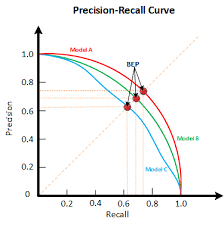
\includegraphics[width=0.38\linewidth]{PR.png}
    \end{figure}


\end{frame}
